\documentclass[12pt]{article}

\usepackage[a4paper,  top=1.3in, bottom=1.4in, left=1.4in, right=1.5in]{geometry}

\usepackage[utf8]{inputenc}
\usepackage[T1]{fontenc}
\usepackage{amsmath}
\usepackage{amsfonts}
\usepackage{amssymb}


\usepackage{graphicx, float}
\usepackage{adjustbox}
\graphicspath{{images/}}

% \renewcommand{\figurename}{Slika}



\renewcommand{\baselinestretch}{1.2} % Line spacing

% Parskip and parindent
\setlength{\parindent}{0pt} % Begin of paragraph indentation
\setlength{\parskip}{1em} % Paragraph spacing

%--- for references ---------
\usepackage[
    backend=biber,
    style=numeric,
    sorting=none
    ]{biblatex}

\addbibresource{bibliography.bib}
\AtBeginBibliography{\vspace*{10pt}}
%----------------------------

%----------- toc ------------------------
\usepackage{tocloft}
\usepackage{fancyhdr}
% \setlength{\cftbeforesecskip}{0pt} % Adjust the spacing before section entries
% \setlength{\cftbeforesubsecskip}{0pt} % Adjust the spacing before subsection entries
%----------------------------------------

\begin{document}

% Title Page
\newgeometry{top=1in, bottom=1in, left=1in, right=1in} % New margins for title page
\begin{titlepage}
    \begin{center}
        
        % add your university logo here
        % negative value moves the logo up
        \vspace*{-1in}
        
\includegraphics[width=0.4\textwidth]{raf_logo.png}

        % set font size to 14pt
        \vspace{1in}
        \Large
        \textbf{Review on the topic of}
        
        % set horizontal margin for the title to 1.5in and center it
        \vspace{1in}
        \Huge
        \textbf{Simultaneous localization and mapping (SLAM)}
        
        \vspace{1in}


            \fontsize{17pt}{17pt}\selectfont
            \textbf{Course: Robotics} \\
            \vspace*{1.5in}
            
            \begin{center}
            \normalsize
            \begin{tabular}{p{0.75\textwidth} p{0.5\textwidth}}
                \fontsize{14pt}{18pt}\selectfont   
                \textbf{Advisor:} & 
            
                \fontsize{14pt}{18pt}\selectfont
                \textbf{Student:} \\
                prof. Miloš Jovanović & Vanja Kovinić \\
            \end{tabular}
            \end{center}

            \vspace*{\fill}

            \normalsize
            Belgrade, 2025.


            
        \end{center}
    \end{titlepage}
    \restoregeometry % Restore original margins

    \newpage
    \newgeometry{top=1.3in, bottom=2.2in, left=1.4in, right=1.4in} % New margins for title page

    \tableofcontents

    \newpage

    \section{Introduction to SLAM}
    \subsection{Definition and Problem Statement}
    \textbf{Simultaneous Localization and Mapping (SLAM)} represents one of the fundamental challenges in robotics. At its core, SLAM addresses a deceptively simple question: 
    \\ \textit{How can a mobile robot build a map of an unknown environment while simultaneously determining its own position within that map?} 
    \\ This seemingly straightforward task embodies a classic \textit{"chicken-and-egg"} problem - to create an accurate map, the robot needs to know its precise location,
    but to determine its location, it needs an accurate map.
    \\ The SLAM problem can be formally defined as the process of constructing or updating a map of an unknown environment while keeping track of an agent's location within it. 
    Mathematically, SLAM estimates both the trajectory of the robot ($X_{1} = {x_1, x_2, \ldots, x_t}$) and the map of the environment ($M$) given the observations ($Z_{1}$) and control inputs ($U_{1}$):
    \[p(X_{1}, M \mid Z_{1}, U_{1})\]
    This joint probability distribution encapsulates the inherent uncertainty in both the robot's position and the environmental map, recognizing that both must be estimated simultaneously.

    \newpage

    The technical challenges of SLAM extend beyond this core problem. Real-world implementations must contend with:
    \begin{enumerate}
        \item \textbf{Sensor limitations}: All sensors provide imperfect measurements with noise, limited range, and potential occlusions.
        \item \textbf{Data association}: Determining whether sensor observations correspond to previously observed landmarks or represent new features.
        \item \textbf{Loop closure}: Recognizing when the robot has returned to a previously visited location, allowing for correction of accumulated errors.
        \item \textbf{Computational efficiency}: Balancing accuracy with real-time performance requirements, especially on platforms with limited computing resources.
        \item \textbf{Environmental dynamics}: Managing changes in the environment, such as moving objects or changing conditions.
    \end{enumerate}

    \begin{figure}[h!]
        \centering
        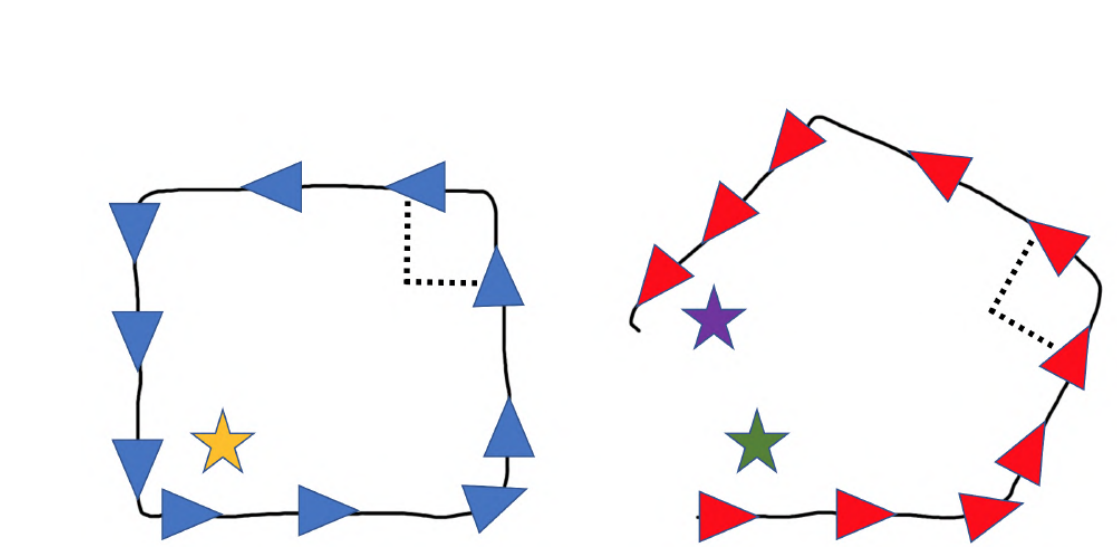
\includegraphics[width=0.8\textwidth]{loop_closure.png}
        \caption{The diagram shows loop closure in robot mapping. When a feature is recognized again (left), a constraint is added to correct the robot's trajectory. 
        If the feature is not recognized (right), errors in the estimated path remain uncorrected. \cite{loop_closure_img}}
        \label{fig:loop_closure}
    \end{figure}

    A successful SLAM system must integrate sensor data over time while accounting for uncertainties and constraints to produce a consistent representation of both the robot's path 
    and the surrounding environment.

    \newpage

    \subsection{Historical Context and Importance in Robotics}
    The development of SLAM techniques represents a crucial milestone in the evolution of autonomous robotics. Before SLAM, robots relied on pre-built maps or simple reactive behaviors, 
    severely limiting their autonomy and usefulness in unknown environments.
    The conceptual foundations of SLAM emerged in the 1980s through seminal work by researchers such as Hugh Durrant-Whyte and John J. Leonard \cite{seminal_paper}, who recognized 
    to the statistical correlations between landmarks in a map. However, the term "SLAM" itself was not coined until the early 1990s.

    The historical progression of SLAM research can be divided into several key phases:

    \begin{enumerate}
        \item \textbf{Early probabilistic approaches (1990s)}: The initial formulation of SLAM using Extended Kalman Filters (EKF) provided the mathematical framework for 
        handling uncertainty in both robot motion and sensing \cite{early_probabilistic_approaches}. These approaches were limited by computational complexity that scaled quadratically with the number of landmarks.
        \item \textbf{Particle filter methods (early 2000s)}: FastSLAM \cite{fast_slam} and other particle filter approaches offered improved performance for nonlinear systems and 
        non-Gaussian noise, enabling more robust implementations.
        \item \textbf{Graph-based optimization (mid-2000s)}: The formulation of SLAM as a sparse graph optimization problem led to more efficient solutions 
        that could handle larger environments and longer trajectories.
        \item \textbf{Visual SLAM systems (2007-2015)}: The incorporation of camera data enabled systems like MonoSLAM \cite{monoslam}, PTAM, and ORB-SLAM \cite{orb_slam}, which could operate 
        using only visual information without specialized ranging sensors.
        \newpage
        \item \textbf{Learning-based approaches (2015-present)}: The integration of deep learning methods has pushed the boundaries of SLAM performance, particularly 
        in feature extraction, depth estimation, and semantic understanding.
    \end{enumerate}

    The introduction of SLAM algorithms effectively gave robots a spatial intelligence - the ability to interpret, map, and navigate previously unseen environments without human guidance.
    Some of the most notable applications of SLAM include:
    \begin{itemize}
        \item \textbf{Autonomous vehicles}: Tesla's FSD system and Waymo's autonomous taxis implement sophisticated SLAM variants that fuse visual data with other sensor modalities. 
        Their ability to navigate complex urban environments relies not just on GPS (which fails in tunnels or urban canyons) but on real-time environmental mapping at centimeter-level precision.
        \item \textbf{Disaster response}: After the Fukushima nuclear disaster, robots equipped with RGBD-SLAM systems entered radiation-contaminated zones inaccessible to humans,
        creating 3D maps that enabled remote assessment of structural damage without endangering human lives \cite{fukushima_disaster}.
        \item \textbf{Domestic robotics}: The evolution of cleaning robots from random bouncers like early Roombas to the systematic path-planners seen in Roborock S7 models 
        illustrates how SLAM transformed consumer robotics from novelties into genuinely useful tools that can efficiently cover complex home layouts.
        \item \textbf{Mixed reality}: Apple's ARKit and Microsoft's HoloLens use visual-inertial SLAM to maintain stable positioning of virtual objects in the physical world, enabling 
        applications from surgical training to architectural visualization that rely on precise spatial registration.
    \end{itemize}

    \begin{figure}[h!]
        \centering
        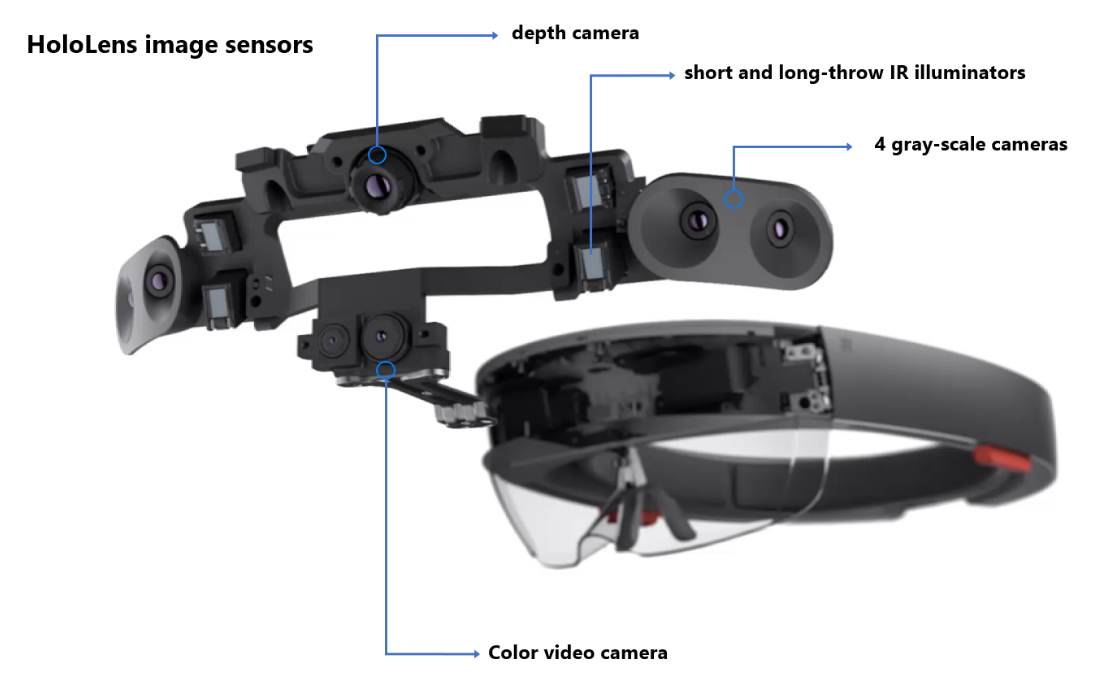
\includegraphics[width=0.7\textwidth]{mcsft_hololens.png}
        \caption{Microsoft HoloLens uses SLAM by fusing data from cameras, depth sensors, and IMUs to simultaneously track the headset’s position and map the environment. 
        This enables accurate placement of virtual objects in the real world for stable and immersive augmented reality experiences.}
        \label{fig:mcsft_hololens}
    \end{figure}


    % \section{Fundamental Challenges in SLAM}
    % \subsection{The Chicken-and-Egg Problem}
    % \subsection{Sensor Limitations and Environmental Factors}
    % \subsection{Loop Closure and Data Association}

    % \section{Classical Approaches to SLAM}
    % \subsection{Filter-Based Methods}
    % \subsection{Graph-Based Optimization}
    % \subsection{Traditional Visual SLAM Systems}

    % \section{Deep Learning in Modern SLAM}
    % \subsection{Learned Features vs. Handcrafted Features}
    % \subsection{End-to-End SLAM Architectures}
    % \subsection{Neural Implicit Representations for Mapping}
    % \subsection{Depth Estimation Networks}

    % \section{Computer Vision Advancements in SLAM}
    % \subsection{Visual Odometry and Place Recognition}
    % \subsection{Semantic SLAM}
    % \subsection{Dynamic Environment Handling}

    % \section{Current Research and Applications}
    % \subsection{Self-Supervised and Few-Shot Learning}
    % \subsection{Real-World Applications}
    % \subsection{Challenges and Future Directions}

    
    \newpage
    \printbibliography[title={References}]
\end{document}